\section{NI.h File Reference}
\label{NI_8h}\index{NI.h@{NI.h}}
{\tt \#include \char`\"{}../simIris/components/interfaces/processor.h\char`\"{}}\par
{\tt \#include \char`\"{}../simIris/components/impl/genericEvents.h\char`\"{}}\par
{\tt \#include \char`\"{}../simIris/data\_\-types/impl/highLevelPacket.h\char`\"{}}\par
{\tt \#include \char`\"{}../simIris/data\_\-types/impl/irisEvent.h\char`\"{}}\par
{\tt \#include \char`\"{}../util/genericData.h\char`\"{}}\par
{\tt \#include \char`\"{}../util/mc\_\-constants.h\char`\"{}}\par
{\tt \#include \char`\"{}request.h\char`\"{}}\par
{\tt \#include \char`\"{}mshr.h\char`\"{}}\par
{\tt \#include $<$fstream$>$}\par
{\tt \#include $<$algorithm$>$}\par


Include dependency graph for NI.h:\nopagebreak
\begin{figure}[H]
\begin{center}
\leavevmode
\includegraphics[width=420pt]{NI_8h__incl}
\end{center}
\end{figure}


This graph shows which files directly or indirectly include this file:\nopagebreak
\begin{figure}[H]
\begin{center}
\leavevmode
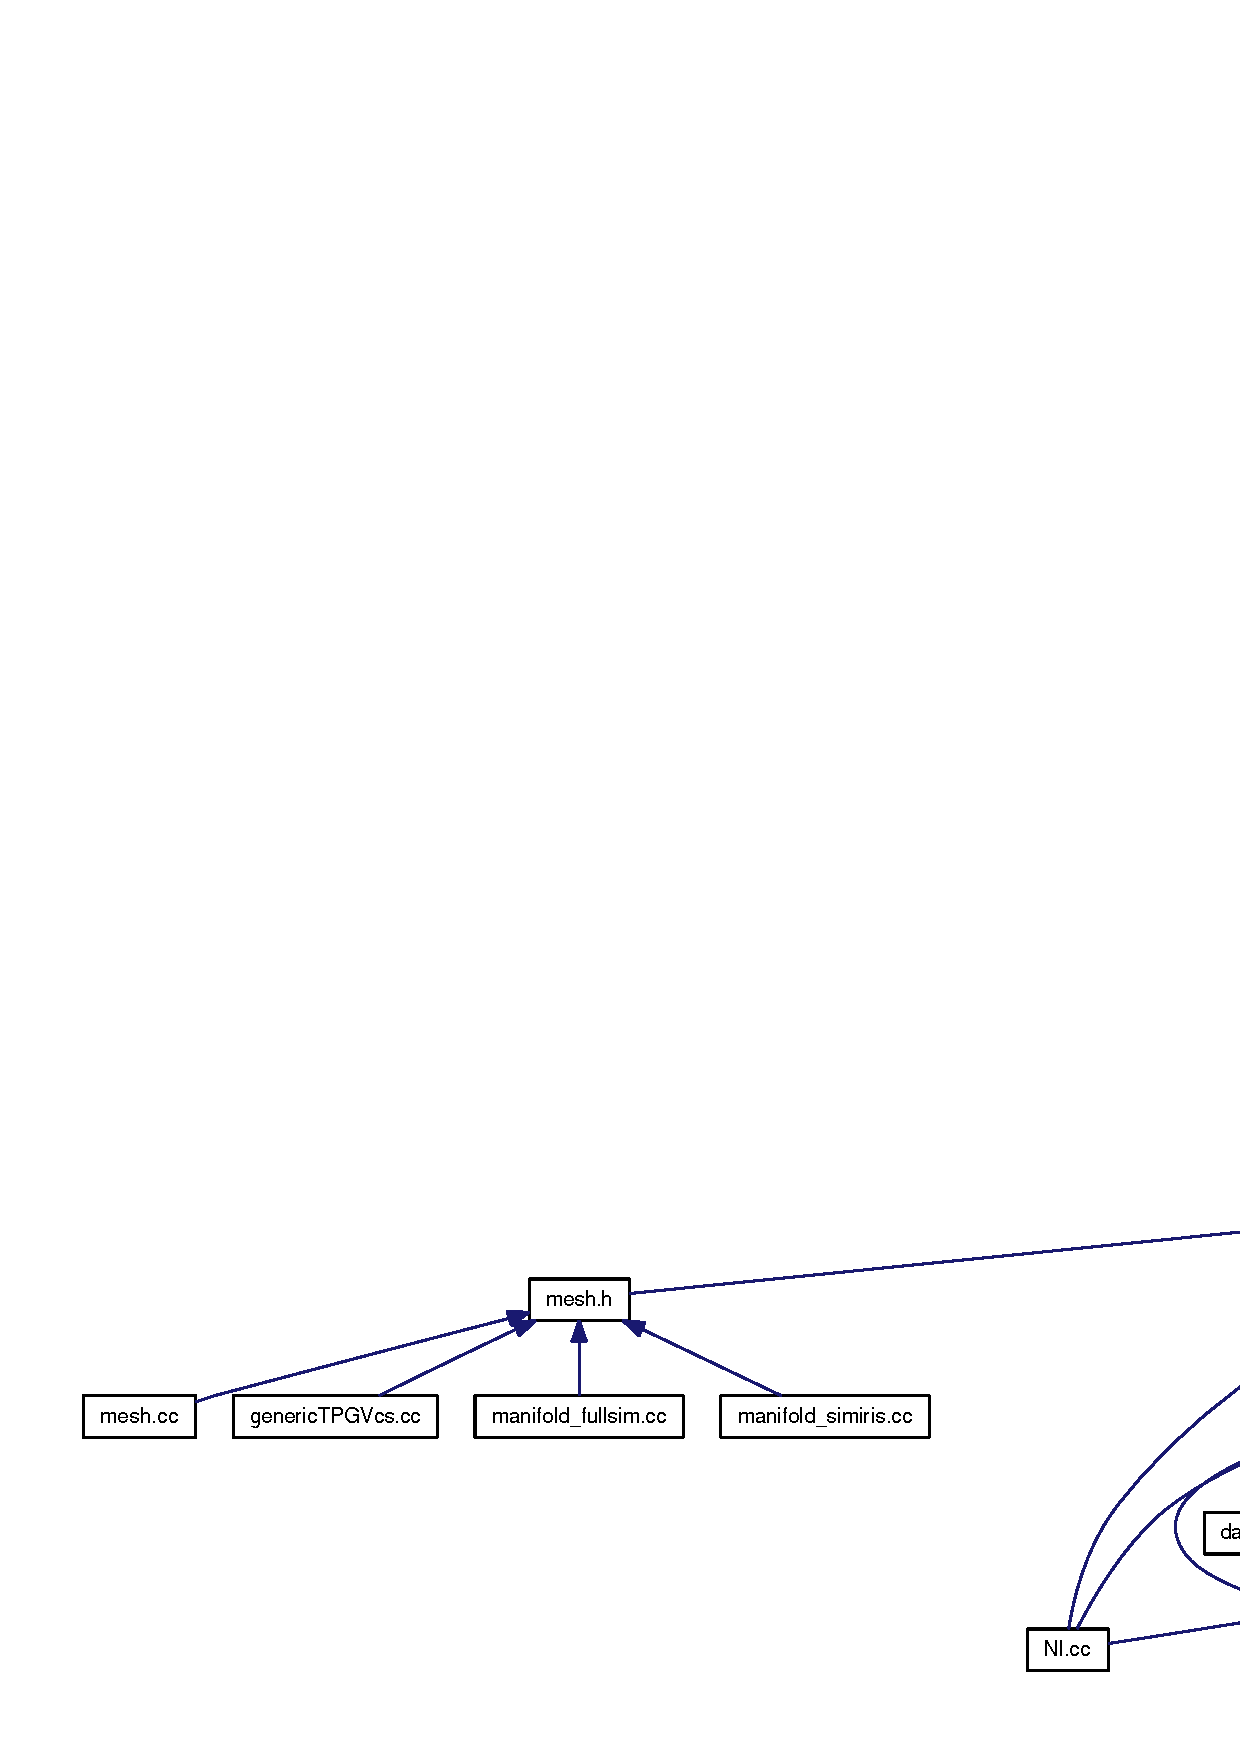
\includegraphics[width=420pt]{NI_8h__dep__incl}
\end{center}
\end{figure}
\subsection*{Classes}
\begin{CompactItemize}
\item 
class {\bf NI}
\end{CompactItemize}
\subsection*{Defines}
\begin{CompactItemize}
\item 
\#define {\bf DEFAULT\_\-RAN\_\-MAX\_\-TIME}~100
\end{CompactItemize}
\subsection*{Variables}
\begin{CompactItemize}
\item 
{\bf uint} {\bf MC\_\-ADDR\_\-BITS}
\item 
{\bf uint} {\bf no\_\-mcs}
\item 
vector$<$ {\bf uint} $>$ {\bf mc\_\-positions}
\end{CompactItemize}


\subsection{Define Documentation}
\index{NI.h@{NI.h}!DEFAULT\_\-RAN\_\-MAX\_\-TIME@{DEFAULT\_\-RAN\_\-MAX\_\-TIME}}
\index{DEFAULT\_\-RAN\_\-MAX\_\-TIME@{DEFAULT\_\-RAN\_\-MAX\_\-TIME}!NI.h@{NI.h}}
\subsubsection[{DEFAULT\_\-RAN\_\-MAX\_\-TIME}]{\setlength{\rightskip}{0pt plus 5cm}\#define DEFAULT\_\-RAN\_\-MAX\_\-TIME~100}\label{NI_8h_95a6218d50e244f6e58b6cca098c1d65}




Definition at line 34 of file NI.h.

\subsection{Variable Documentation}
\index{NI.h@{NI.h}!MC\_\-ADDR\_\-BITS@{MC\_\-ADDR\_\-BITS}}
\index{MC\_\-ADDR\_\-BITS@{MC\_\-ADDR\_\-BITS}!NI.h@{NI.h}}
\subsubsection[{MC\_\-ADDR\_\-BITS}]{\setlength{\rightskip}{0pt plus 5cm}{\bf uint} {\bf MC\_\-ADDR\_\-BITS}}\label{NI_8h_5ef66c602b93d3db97dac0d557e7c84b}




Definition at line 37 of file config\_\-constants.h.\index{NI.h@{NI.h}!mc\_\-positions@{mc\_\-positions}}
\index{mc\_\-positions@{mc\_\-positions}!NI.h@{NI.h}}
\subsubsection[{mc\_\-positions}]{\setlength{\rightskip}{0pt plus 5cm}vector$<${\bf uint}$>$ {\bf mc\_\-positions}}\label{NI_8h_f58ebe62f79b2e470f0cb7da0f7a7ea5}




Definition at line 46 of file config\_\-params.h.\index{NI.h@{NI.h}!no\_\-mcs@{no\_\-mcs}}
\index{no\_\-mcs@{no\_\-mcs}!NI.h@{NI.h}}
\subsubsection[{no\_\-mcs}]{\setlength{\rightskip}{0pt plus 5cm}{\bf uint} {\bf no\_\-mcs}}\label{NI_8h_56d27d790e05179f3787fce80d802d04}




Definition at line 31 of file config\_\-params.h.